\subsubsection{Paginaci\'on de las tareas}

Para la paginaci\'on de tareas se necesitaron los siguientes m\'odulos por cada tarea:
\begin{itemize}
 \item Inicializar un directorio de p\'aginas con 5 entradas, 4 para el Kernel iguales a las descriptas en el ejercicio 3 (es decir, identity mapping) 
 y dos para direccionar a las p\'aginas de c\'odigo y pilas de cada tarea. Este Page directory est\'a definido en la direccion 0x40000000
 \item Dentro de la Page Table de las tareas se encuentran definidas las entradas de cada p\'agina de la tarea. 
\end{itemize}

Con el fin de simplificar la cantidad de pasos, las direcciones fisicas de las paginas cada tarea estaran mapeadas en arrays externos. De esta forma no
tendremos que buscar dentro de la GDT para buscar una direccion fisica a la hora de hacer otras operaciones, que puede ser costoso en cuestiones de tiempo
y dejar un codigo poco claro.

A diferencia del ejercicio anterior, como en este caso estamos mapeando tareas, estas se diferencian de las p\'aginas de Kernel en que
los attributos que utilizan son diferentes, es decir, las tareas al correr en nivel 3 requieren que sus Page Directory entries y sus
Page table entries posean U/S = 1. De lo contrario no puedo acceder a esas p\'aginas como nos lo demostro\'o nustra experiencia en la
implementaci\'on.

El siguiente esquema explica mas simplemente lo nombrado anteriormente. Tener en cuenta que esto debe realizarse por cada tarea y que si
bien cada una est\'a mapeada al mismo lugar, la base del Page Directory es distinto para cada tarea, provocando que cada una tenga su
propio mapeo. %Para empezar, page directory entry que corresponde a la tarea, es la 0x100 ya que 0x40000000 es una direccion virtual entonces
%la tenemos que decodificar como 

%\begin{center}
%  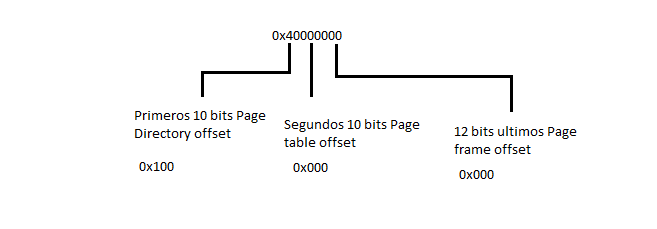
\includegraphics[scale=0.6]{imagenes/ComoDividoVirtual.png} 
%\end{center}

%Y Luego de esto el esquema de paginaci\'on nos quedar\'ia algo as\'i:

%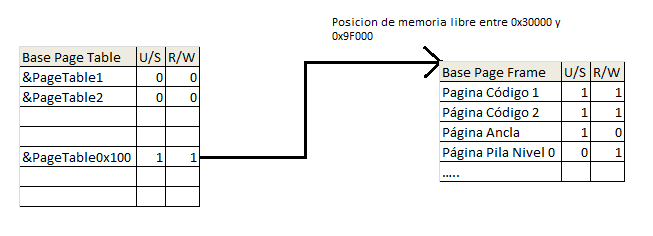
\includegraphics[scale=0.6]{imagenes/paginacionTareas.png}

Cabe destacar que para poder cumplir con los ejercicios siguientes, una tarea IDLE va a tener que ser mapeada al comienzo de la paginaci\'on
de lo contrario, no tener una tarea mapeada me imposibilita arrancar el sistema de scheduling que ser\'a introducido mas adelante.\footnote{Ver
secci\'on Ejercicio 7, Scheduling.}
